\documentclass[t, 10pt, handout, aspectratio=169]{beamer}
\usepackage{tikz}
\usepackage{pgfplots}
\usepackage{booktabs}
\usepackage{graphicx}
\usepackage{ragged2e} % Using the standard package
\pgfplotsset{compat=1.14}

% Use the KU theme as requested
\usetheme[color=blue,framenumber,totalframenumber, footline, footertext]{KU}

% --- Metadata ---
\title[Knowledge-and-Language]{Knowledge-and-Language}
\subtitle{A Bilingual Recipe Assistant Combining a Knowledge Graph, Lightweight NLP, and LLMs}
\author[M. Castela, M. Martins]{Miguel Castela \and Miguel Martins}
\institute[UC]{University of Coimbra \\ Department of Informatics Engineering}

\footertext{Knowledge-and-Language 2025/2026}
\date{\today}

\begin{document}

% --- Title Slide ---
\begin{frame}
  \titlepage
\end{frame}

% --- Outline ---
\begin{frame}{Outline}
  \tableofcontents
\end{frame}

% --- Section 1: Introduction ---
\section{Introduction}
\begin{frame}{Motivation \& Core Challenge}
  \begin{columns}
    \column{0.6\textwidth}
      \textbf{Context:}
      \begin{itemize}
        \item Recipe retrieval is often limited to keyword matching.
        \item Users have complex, multi-criteria constraints (dietary, time, ingredients).
        \item Multilingual support (PT/EN) is challenging for structured data.
      \end{itemize}
      
      \vspace{1em}
      \textbf{Objective:}
  \end{columns}
\end{frame}


\section{Objective}
\begin{frame}{Objective}
  \begin{columns}
    \column{0.6\textwidth}
      \textbf{Context:}
      \begin{itemize}
        \item Develop a \textbf{Bilingual Assistant} that understands intent.
        \item Combine the \textbf{precision of Knowledge Graphs (KG)} with the \textbf{fluency of LLMs}.
      \end{itemize}
      
      \vspace{1em}
      \textbf{Objective:}
  \end{columns}
\end{frame}

% --- Section 2: Architecture ---
\section{System Architecture}
\begin{frame}{System Pipeline}
  \textbf{Hybrid Retrieval: SPARQL (KG) + FAISS (Vector Search)}
  
  \vspace{0.5em}
  \begin{itemize}
    \item \textbf{Input:} User query (Portuguese or English).
    \item \textbf{NLP Layer:} Intent classification (\textbf{BERT}) + Entity Extraction (\textbf{spaCy/RapidFuzz}).
    \item \textbf{Retrieval:} SPARQL for structured data + FAISS index on descriptions.
    \item \textbf{Generation:} LLM (\textbf{Groq API}) generates summarized results bilingually.
  \end{itemize}
\end{frame}

% --- Section 3: Key Components ---
\section{Key Components}
\subsection{NLP Pipeline \& Time Parsing}
\begin{frame}{NLP: Intent \& Entity Extraction}
  \begin{columns}
    \column{0.5\textwidth}
      \begin{block}{1. Intent Classification}
        \begin{itemize}
          \item Fine-tuned \texttt{bert-base-multilingual-cased}.
          \item Classes include: \texttt{list\_by\_ingredient}, \texttt{list\_by\_time}, \texttt{find\_recipe}, etc..
          \item Achieved $\sim$92\% Intent Accuracy on test queries.
        \end{itemize}
      \end{block}
      
      \begin{block}{2. Entity Extraction \& Linking}
        \begin{itemize}
          \item Uses \texttt{RapidFuzz} for fuzzy matching against KG labels.
          \item High entity linking accuracy using similarity thresholds (Ing=85, Tag=90).
        \end{itemize}
      \end{block}
  \end{columns}
\end{frame}


\section{Key Components}
\subsection{NLP Pipeline \& Time Parsing}
\begin{frame}{NLP: Intent \& Entity Extraction}
  \begin{columns}
\column{0.5\textwidth}
      \begin{block}{3. Time Constraint Handling}
        \begin{itemize}
          \item \textbf{Challenge:} User descriptions are highly variable and ambiguous (e.g., "1h20", "under 10 minutes").
          \item \textbf{Solution:} Layered numeric parsing, translation normalization, and regex for exact/maximum duration.
          \item Time Parsing is robust and handles typos.
        \end{itemize}
      \end{block}
  \end{columns}
\end{frame}

\subsection{SPARQL Query Functions}
\begin{frame}{SPARQL Functions: Intent-to-Query Mapping}
  \justifying
  Each user intent is mapped to a specific SPARQL query function, filled with extracted entities, to retrieve structured data from the KG.

  \begin{columns}
    \column{0.5\textwidth}
      \textbf{Functions for Specific Recipes or Values:}
      \begin{itemize}
        \item \textbf{Retrieve Ingredients} (\texttt{retrieve\_ingredients}) 
        \item \textbf{Find Recipe} (\texttt{find\_recipe}) 
        \item \textbf{Get Preparation Time} (\texttt{get\_prep\_time})
      \end{itemize}
      % CORRECT PATHS with folder and fixed filenames:
      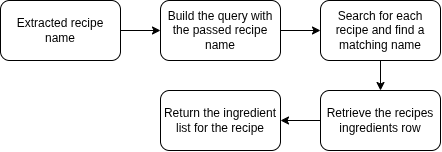
\includegraphics[width=0.8\linewidth, height=0.2\textheight, keepaspectratio]{cl-drawio/cl-retrieve_ingredients.drawio.png}
      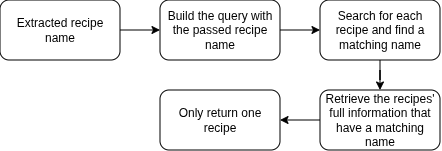
\includegraphics[width=0.8\linewidth, height=0.2\textheight, keepaspectratio]{cl-drawio/cl-find_recipe.drawio.png}
      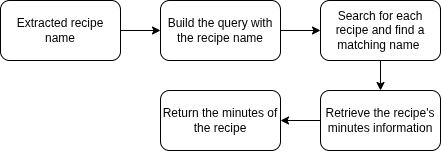
\includegraphics[width=0.8\linewidth, height=0.2\textheight, keepaspectratio]{cl-drawio/cl-get_prep_time.drawio.png}
    \column{0.5\textwidth}
      \textbf{Functions for List Retrieval:}
      \begin{itemize}
        \item \textbf{List by Tag} (\texttt{list\_by\_tag}) 
        \item \textbf{List by Ingredient} (\texttt{list\_by\_ingredient}) 
        \item \textbf{List by Time} (\texttt{query\_by\_max/exact\_minutes}) 
      \end{itemize}
      % CORRECT PATHS with folder and fixed filenames:
  \end{columns}
  
\end{frame}


\begin{frame}{SPARQL Functions: Intent-to-Query Mapping}
  \justifying
  Each user intent is mapped to a specific SPARQL query function, filled with extracted entities, to retrieve structured data from the KG.

      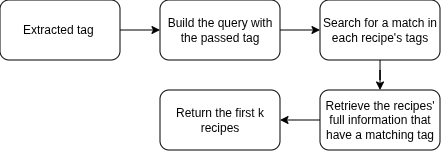
\includegraphics[width=0.8\linewidth, height=0.2\textheight, keepaspectratio]{cl-drawio/cl-list_by_tag.drawio.png}
      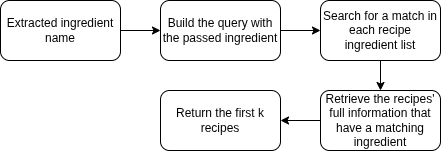
\includegraphics[width=0.8\linewidth, height=0.2\textheight, keepaspectratio]{cl-drawio/cl-list_by_ingr.drawio.png}
      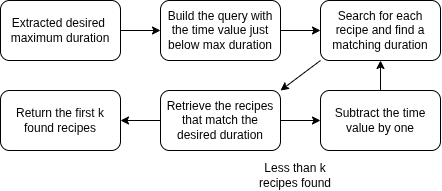
\includegraphics[width=0.8\linewidth, height=0.2\textheight, keepaspectratio]{cl-drawio/cl-get_max_time.drawio.png}
  
\end{frame}

% --- Section 4: Results & Conclusion ---
\section{Results \& Conclusion}
\begin{frame}{Experimental Results Summary}

  \vspace{1em}
  \textbf{Key Findings:}
  \begin{itemize}
    \item \textbf{Bilingual Consistency:} Improved translation normalization ensured stable and deterministic results across PT/EN queries.
    \item \textbf{RAG Impact:} RAG showed little measurable impact; the KG already provided comprehensive, relevant information.
    \item \textbf{Hard Queries:} For creative queries, the LLM used retrieved data to ask clarifying questions, guiding the user back to valid intents.
  \end{itemize}
\end{frame}

\begin{frame}{Conclusion \& Future Work}
  \begin{itemize}
    \item \textbf{Summary:}
      \begin{itemize}
        \item Successfully integrated a KG with LLMs for a robust bilingual assistant.
        \item Solved specific NLP challenges in entity linking, time parsing, and translation consistency.
      \end{itemize}
    
    \vspace{1em}
    \item \textbf{Future Directions:}
      \begin{itemize}
        \item \textbf{Expand KG:} Include more recipes and nutritional facets.
        \item \textbf{Personalization:} Implement user profiles for dietary restrictions.
        \item \textbf{Evaluation:} Add automated metrics (BLEU/ROUGE) and reinforcement learning from human feedback (RLHF).
      \end{itemize}
  \end{itemize}
\end{frame}

\begin{frame}[plain]

\centering
\Huge \textcolor{structure.fg}{Thank You!} \
\vspace{1em}
\large Questions?
\end{frame}

\end{document}